\documentclass{tufte-handout}

%\geometry{showframe}% for debugging purposes -- displays the margins

\usepackage{amsmath}

% Set up the images/graphics package
\usepackage{graphicx}
\setkeys{Gin}{width=\linewidth,totalheight=\textheight,keepaspectratio}
\graphicspath{{graphics/}}

\title{Endocrine and Hypothalamic Control of Appetite}
\author{Dave Bridges, Ph.D.}
%\date{24 January 2009}  % if the \date{} command is left out, the current date will be used

% The following package makes prettier tables.  We're all about the bling!
\usepackage{booktabs}

% The units package provides nice, non-stacked fractions and better spacing
% for units.
\usepackage{units}

% The fancyvrb package lets us customize the formatting of verbatim
% environments.  We use a slightly smaller font.
\usepackage{fancyvrb}
\fvset{fontsize=\normalsize}

% Small sections of multiple columns
\usepackage{multicol}

% Provides paragraphs of dummy text
\usepackage{lipsum}

% These commands are used to pretty-print LaTeX commands
\newcommand{\doccmd}[1]{\texttt{\textbackslash#1}}% command name -- adds backslash automatically
\newcommand{\docopt}[1]{\ensuremath{\langle}\textrm{\textit{#1}}\ensuremath{\rangle}}% optional command argument
\newcommand{\docarg}[1]{\textrm{\textit{#1}}}% (required) command argument
\newenvironment{docspec}{\begin{quote}\noindent}{\end{quote}}% command specification environment
\newcommand{\docenv}[1]{\textsf{#1}}% environment name
\newcommand{\docpkg}[1]{\texttt{#1}}% package name
\newcommand{\doccls}[1]{\texttt{#1}}% document class name
\newcommand{\docclsopt}[1]{\texttt{#1}}% document class option name

\begin{document}

\maketitle% this prints the handout title, author, and date

\begin{abstract}
\noindent This lecture covers endocrine control of appetite.  We will discuss the neural circuitry that regulates appetite and how peripheral signals from the gut, pancreas and adipose tissue can modify feeding behavior.  This lecture covers the following pages in the textbook: 571-4 \cite{Widmaier2013}.  
\end{abstract}

\tableofcontents

\pagebreak

\section{Learning Objectives}
For this lecture, the learning objectives are:
\begin{itemize}
\item Describe the appetite-regulating hormones secreted from the gut, how they are regulated and under what conditions they are released.
\item Describe the AgRP/POMC circuit and its relationship to both circulating factors and neuropeptides.
\item Understand the relationship between adipose mass and appetite regulation, including how adipokines are regulated and what role they play.
\item List the effects of insulin on appetite and what the neurological targets of insulin are.
\item Describe the role of the blood-brain barrier in the regulation of appetite and how it is altered in obesity.
\item Describe how hypothalamic feeding circuits integrate with other pleasure and reward circuits in the brain.
\item Explain how neuroendocrine obesity differs from idiopathic obesity and how they might be treated in different ways.

\end{itemize}

\section{Hypothalamic Control of Appetite}

Appetite regulation is a complex behavior, requiring both peripheral and cognitive inputs.  The most important site for appetite regulation is within the hypothalamus, which as we discussed, is the most important location by which the central nervous system and the endocrine system intersect.  

\subsection{Neural Circuitry that Regulates Appetite}

The primary neural circuit that regulates appetite is the POMC/AgRP system within the arcuate nucleus of the hypothalamus.  Typically POMC\sidenote{Occasionally called CART neurons} signal to other parts of the brain to reduce food-seeking behavior.  This signaling can be repressed by a second set of neurons, called AgRP\sidenote{These are sometimes called NPY neurons.  These induce food seeking behavior when active.} neurons, other synaptic inputs or blood-borne signals.  This circuit is shown below in Figure \ref{fig:agrp-pomc}, modified from \cite{Bell2005}.

\begin{figure}
\centering
  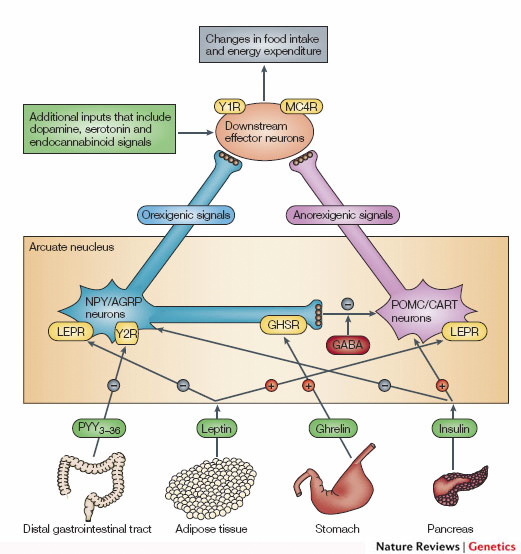
\includegraphics[width=0.8\textwidth]{figures/agrp-pomc}
  \caption{Neural circuitry of appetite regulation}
    \label{fig:agrp-pomc}
\end{figure}

When they fire, POMC neurons release several neurotransmitters which regulate feeding and and mood.  One of the most important of these is $\alpha$-MSH, a \textit{POMC} derived peptide hormone which binds to receptors in the PVN\sidenote{paraventricular nucleus} of the hypothalamus.  Downstream of the $\alpha$-MSH receptor\sidenote{known as the melanocortin 4 receptor or \textit{MC4R}}, food intake is suppressed and energy expenditure processes are activated.

\newthought{In addition to $\alpha$-MSH}, another \textit{POMC}-derived peptide, named $\beta$-endorphin is also released in response to feeding.  Endorphins\sidenote{these are endogenous opiods} function on the reward centers of the brain and mediate the hedonistic response to food.

\subsection{Glucose and Fatty Acid Sensing}

Since the blood-brain barrier of the hypothalamus is partially exposed to systemic blood factors, the hypothalamus can directly sense both glucose and fatty acids levels in the blood.  In the case of glucose, a glucose/K\textsuperscript{+} co-transporter can cause depolarization of POMC neurons\cite{Parton2007}.  There are also glucose-responsive and fatty-acid responsive neurons in the subfornicular organ and area postrema\sidenote{These are two other brain regions which can sense blood factors directly, due to absent or weakened blood-brain barrier}, which can synapse to POMC neurons and inhibit them indirectly.

\newthought{Aside from direct sensing of metabolites}, there are several hormones which can modify the POMC/AgRP circuit in order to suppress or promote appetite.  These include adipose, gut and pancreatic derived hormones, which we will discuss below.

\section{Hormonal Regulation of Appetite}

Conceptually, there are several reasons for why it would be beneficial for the the periphery to stimulate or suppress appetite.  One example is that in times of acute stress, adrenaline can cause anorexia\sidenote{reduced appetite}\cite{RUSSEK1962} as a way to focus on escaping from the immediate stressor.  The major endocrine factors which modulate appetite are summarized below in Table \ref{tab:appetite-hormones}:

\begin{table}
  \centering
  \begin{tabular}{llll}
    \toprule
    Hormone & Source & Signal & Response \\
    \midrule
    Adrenaline & Adrenal medulla & Acute stress & Anorexic \\
    Insulin & Pancreatic $\beta$ cells & Hyperglycemia & Anorexic \\
    PYY$_{3-36}$ & L-Cells of GI Tract & Food Intake & Anorexic \\
    Ghrelin & Ghrelin Cells in Stomach & Stomach Stretch & Orexigenic \\
    Leptin & Adipocytes & Adipocyte Size & Anorexic \\
    \bottomrule
  \end{tabular}
  \caption{Summary of the major appetite regulating endocrine hormones.}
  \label{tab:appetite-hormones}
  %\zsavepos{pos:normaltab}
\end{table}


\subsection{Pancreatic Regulation of Appetite}

In the previous lecture, we discussed how the pancreas releases insulin in response to elevated blood glucose levels.  If able to pass the blood-brain barrier\sidenote{This process requires a transporter.}, insulin can also act on the brain as an appetite suppressing signal.  There are insulin receptors both on POMC and AgRP neurons, which through mechanisms that are currently unclear, co-ordinately reduce food intake. If brain insulin receptors are genetically deleted, mice over-eat and become obese\cite{Bruning2000} 

\subsection{Ghrelin, PYY and the Gut Hormones}

There are two major hormones released from the gastrointestinal tract that regulate food intake, ghrelin and  PYY.  

Normally, ghrelin is released from specialized cells in the stomach.   Ghrelin activates GPCR signaling\sidenote{Gq, but the mechanisms by which ghrelin regulates neuronal firing are not clear.} on the AgRP neurons of the arcuate nucleus, resulting in decreased activation of POMC\sidenote{Due the release of AgRP inhibition.} and MC4R cells and increased food intake.  When the stomach is stretched\sidenote{As in after a meal} ghrelin release is inhibited\sidenote{Just like renin release is blocked by reduced stretch of JG cells.}.  In this way, the stomach can signal to the brain to prevent further food intake.

\newthought{PYY\sidenote{Peptide YY} is a peptide hormone released from enteroendocrine cells} of the colon called L-cells.  The release of this peptide is stimulated by elevated nutrients in the colon, but also can be stimulated by release of upper-GI tract hormones such as CCK\sidenote{see Dr. Johnson's lectures for more information on this}.  PYY has several roles in digestion, including stimulating exocrine release of pancreatic enzymes and modulating GI tract motility.  In addition to these effects, PYY also has potent appetite suppression effects.  PYY signals via AgRP neurons, inhibiting their normal pro-feeding function.  The mechanisms by which this GPCR-dependent signaling alters AgRP firing is still unclear.

\subsection{Leptin and the Adipokines}

One of the most surprising sources of hormones, identified in the past 20 years or so is leptin.  In the 1950s, a naturally occuring mutant mouse was found that had extreme susceptibility to obesity due to unrestrained over-eating\cite{Ingalls1950}.  It took almost 50 years, but eventually the location of this mutation was identified to be a novel secreted polypeptide, exclusively expressed in adipose tissue\cite{Zhang1994}.  Since that time, several other hormones have been identified as secreted from adipose tissue\sidenote{Collectively these are known as adipokines.}.

\newthought{Leptin's primary role is to inhibit food intake in the brain.}  Leptin signals through JAK/STAT receptors in both POMC and AgRP neurons.  When adipose tissue expands, and animals are fed, leptin release is elevated.  This causes transcriptional and post-translational changes in both POMC and AgRP neurons, which result in reduced food intake.

\subsection{Obesity, Negative Feedback and the Role of the Blood Brain Barrier}

The identification of appetite suppressing hormones such as PYY and Leptin lead to a lot of excitement in the obesity field.  It was hoped in the same way that exogenous insulin "cured" type I diabetes, obesity could be treated by administration of these hormones.  Unfortunately this has not proven to be efficient, for the same reason that providing insulin is minimally effective in type II diabetes.  In both cases, the circulating hormone is already at elevated levels in the disease state and negative feedback mechanisms have been activated.  This means, that further leptin is ineffective, because in obese states, people are normally already effectively leptin resistant.

\newthought{Among these negative feedback mechanisms} are receptor desensitization, but this problem is further exacerbated by the presence of the blood-brain barrier.  Many of these hormones require transport mechanisms to cross into the hypothalamus, and in the case of at least insulin and leptin, this transport is reduced in obesity.

\subsection{Treatment of Neuroendocrine Obesity}

The majority of obese individuals do not have a single-gene defect that results in their phenotype, but a small subset of patients do have a defined genetic lesion.  Many of these mutations are in these described endocrine pathways (see Table \ref{tab:genes-obesity}).

\begin{margintable}[+1cm]
  \centering
  \begin{tabular}{lll}
    \toprule
    Gene & Role & Incidence \\
    \midrule
    \textit{LEP} & Leptin & rare \\
    \textit{LEPR} & Leptin Receptor & 2-5\% \\
    \textit{POMC} & Several hormones & rare \\
    \textit{MC4R} & $\alpha$-MSH Receptor & 2-5\% \\
    \bottomrule
  \end{tabular}
  \caption{Selected monogenic disorders of obesity.  Percentages are the percent of obese individuals}
  \label{tab:genes-obesity}
  %\zsavepos{pos:normaltab}
\end{margintable}

These patients are suffering from an etiologically distinct disease, relative to the general population.  They have a specific endocrine defect that is in principle able to be repaired.  As an example, the patients with \textit{LEP} mutations \emph{can} be effectively treated with exogenous leptin\cite{Farooqi1999}.

This was the last informational lecture in this series, in our final lecture we will discuss a clinical case from the textbook, putting some of the principles and hormones we have learned to practice.

\listoffigures
\listoftables

\bibliography{library}
\bibliographystyle{plainnat}



\end{document}
